\documentclass{article}[12pt]
\usepackage[utf8]{inputenc}
\usepackage[a4paper, total={15.5cm, 23cm}]{geometry}
\usepackage{multicol}
\usepackage{amsmath}
\usepackage{mathtools}
\usepackage{graphicx}
\usepackage{titlesec}
\usepackage[parfill]{parskip}

\usepackage{bigfoot}
\DeclareNewFootnote{default}
\DeclareNewFootnote{B}[fnsymbol]
\DeclareNewFootnote{C}[Roman]
\MakeSortedPerPage{footnoteB}
\newcommand{\pro}[1]{\footnoteB{\textit{dice il prof}: #1}}
\newcommand{\gab}[1]{\footnoteC{\textit{consiglia Gabriel}: #1}}

\begin{document}
\section{Modellazione}

\subsection{Modelli notevoli}

\begin{multicols}{2}

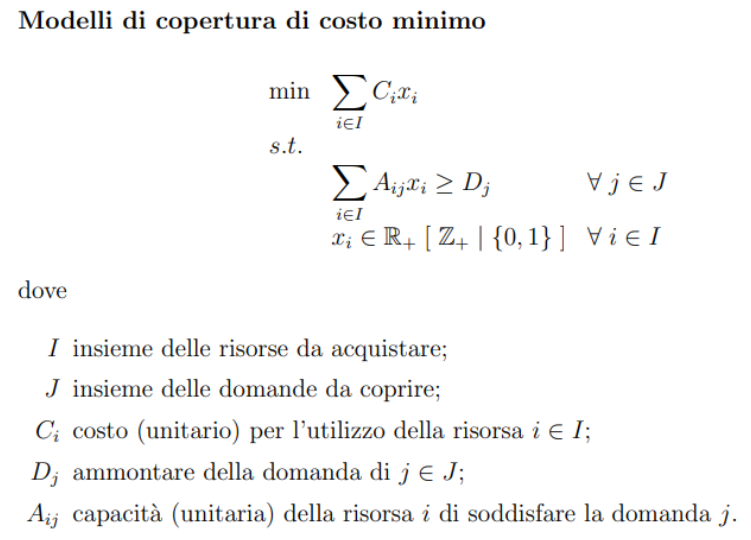
\includegraphics[width=\linewidth]{img/copertura-costo-minimo.png}

\includegraphics[width=\linewidth]{img/mix-ottimo.png}
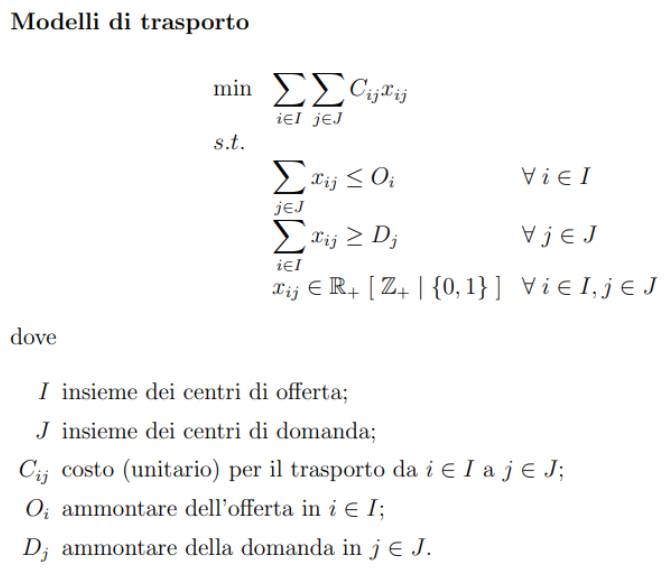
\includegraphics[width=\linewidth]{img/trasporti.png}
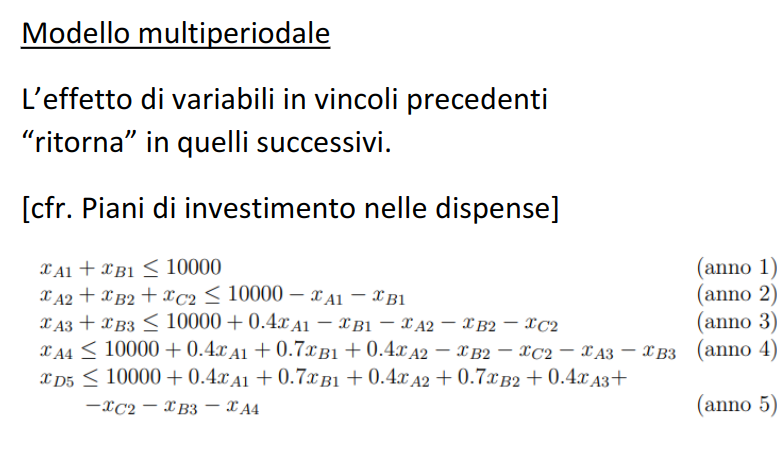
\includegraphics[width=\linewidth]{img/multiperiodale.png}

\end{multicols}
\subsection{Passaggi}
\begin{enumerate}
    \item Individuare le variabili decisionali;
    \item definire la funzione obiettivo;
    \item iniziare a stendere i vincoli non nella parte dei "tenendo conto che:";
    \item iniziare a stendere almeno un vincolo dell'elenco puntato che propone il professore\pro{Almeno uno o due di questi vincoli sono comodi per scrivere il resto del modello};
    \item Scrivere il resto dei vincoli;
    \item Scrivere i domini.
\end{enumerate}

\subsubsection{Individuazione delle variabili decisionali}
Queste variabili sono solitamente a uno o due indici\gab{Spesso le variabii a due indici fanno danni, meglio mettere più variabili ad un indice se possibile.}.
Diventa invece preferibile mettere a due indice quando è evidente dal problema che servono entrambe due colonne di una tabella\footnote{Nel problema dei trasporti solitamente usiamo due indici.}.

Un'altra cosa a cui fare attenzione è la scrittura dei vincoli in cui un \textit{"Indipendentemente da"} ci fa capire che probabilmente avremo bisogno di una variabile ad un indice solo e non due.

\subsubsection{Definizione della funzione obiettivo}
La funzione obiettivo \textbf{DEVE} essere lineare\footnote{Se non è lineare, allora non è un problema di programmazione lineare. (detto più brevemente anche problema di PL).}.

É importante fare molta attenzione a non moltiplicare due variabili, anche se una delle due variabili è binaria.

\subsubsection{Vincoli}

Anche i vincoli \textbf{DEVONO} essere lineari.

\paragraph{I vincoli logici} Se ho vincoli logici, ad esempio "posso decidere se fare X cosa" devo inserire una variabile binaria. Per questi vincoli devo:
\begin{itemize}
    \item definirli nel dominio delle varibili binarie;
    \item attivare\footnote{Linearizzare un modello evitando i termini quadratici.} la variabile utilizzando il \textit{Big-M}
\end{itemize} 

\paragraph{Costi fissi} In questo caso va aggiunto un termine moltiplicativo a tutte le variabili decisionali legate per quantità.
\paragraph{Almeno tot}\footnote{Almeno un treno tra gli $y$ treni deve partire $\sum_{i=1}^{n}y_i >= 1$ } Se il vincolo è logico uso $y_1+y_2+y_n >= \text{Il valore del vincolo}$ con $y$ variabile binaria legata a \textit{Big-M}.

Se il vincolo è di quantità uso: $x_1+x_2+x_n >= \text{Il valore del vincolo}$ con $x$ variabile di quantità.

\paragraph{Al massimo tot} Se il vincolo è logico uso $y_1+y_2+y_n <= \text{Il valore del vincolo}$ con $y$ variabile binaria legata a \textit{Big-M}.

Se il vincolo è di quantità uso $x_1+x_2+x_n <= \text{Il valore del vincolo}$ con $x$ variabile di quantità.

\subsubsection{Consigli ulteriori di Gabriel}
\begin{itemize}
    \item 
    Se si sta scrivendo un vincolo e non si capisce bene come scriverlo, probabilmente può essere scritto più semplicemente, anche ripensando alle variabili che lo compongono;
    \item risemplificare e considerare i punti detti è molto utile.
\end{itemize}


\subsubsection{Consigli di Ale}

\begin{itemize}
    \item Rileggere un paio di volte il problema prima di scrivere qualsiasi cosa;
    \item quando si scrive un vincolo cercare di cancellare a matita la parte che lo descrive per evitare di ripassarci sopra prima della lettura finale;
    \item rileggere tutto alla fine per vedere se si è coperto tutto e per controllare di non aver aggiunto situazioni non lineari involontariamente.
\end{itemize}




\section{Foglio esame Ale}
\pagebreak

\titleformat*{\subsection}{\fontsize{10}{12} \bfseries}
\titleformat*{\subsubsection}{\fontsize{8}{12} \bfseries}

\fontsize{8}{12}\selectfont

\newgeometry{left=0.5cm,right=0.5cm,top=0.5cm,bottom=0.5cm}
\begin{multicols}{2}

\subsection*{Programmazione lineare e modellazione}
\begin{enumerate}
    \item Cosa devo decidere;
    \item Quale è l'obiettivo;
    \item Come sono caratterizzate le soluzioni ammissibili(Vincoli del problema);
    \item Specificare il valore delle variabili.
\end{enumerate}
Se aggiungo variabili logiche si attivano con $x_i <= M y_i$.

$M$ è grande come il massimo raggiungibile dalla $x_i$ oppure dalla somma delle $X$ se queste sono attivate assieme.

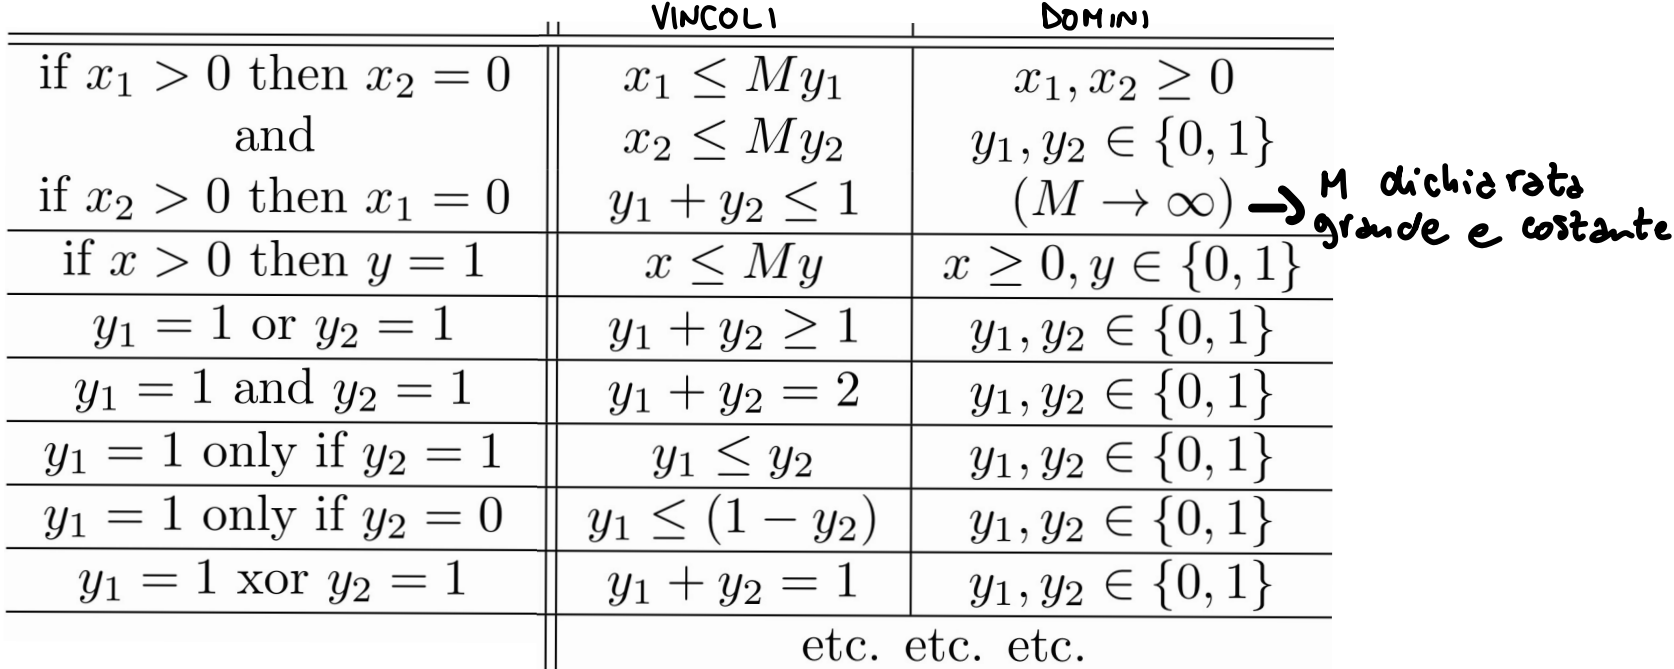
\includegraphics[width=0.9\linewidth]{img/vincoli_pl.png}

\begin{itemize}
    \item Linearità;
    \item Valori spuri;
\end{itemize}

\subsection*{Simplesso}
Convergenza in al più $\binom{n}{m}$ iterazioni;

Forma standard


\subsection*{Problemi di CCPD}
\begin{enumerate}
    \item Verifico l'ammissibilità del problema primale;
    \item Costruisco il problema duale con le relative regole;
    \item Costruisco usando l'enunciato di CCPD il problema duale;
    \item Metto a sistema le condizioni valide e ricavo gli $u_i$;
    \item Verifico l'ammissibilità del problema duale;
    \item Traggo le conclusioni.
    
    \fontsize{6}{12}\selectfont
    $
    \begin{rcases}
    x & \textrm{è ammissibile primale(verifica 1)}\\
    u & \textrm{è ammissibile duale(verifica 5)}\\
    x,u & \textrm{sono in scarti complementari(costruzione 3)}
    \end{rcases} 
    \Rightarrow
    x,u \quad \textrm{sono ottime}      
    $
    \fontsize{8}{12}\selectfont

    \item Posso verificare che $z,w$ ottime sono coincidenti.
\end{enumerate}

\subsection*{Regole di trasformazione CCPD}
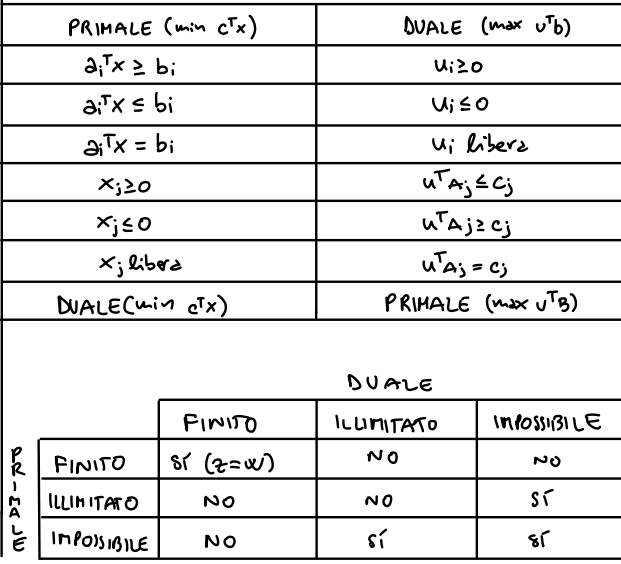
\includegraphics[width=0.9\linewidth]{img/trasformazioneCCPD.png}
\subsection*{Branch and bound}
\subsubsection*{Problemi di minimo}
\subsubsection*{Problemi di massimo}


\end{multicols}
\restoregeometry
\end{document}